\newpage
\begin{song}{title={Skarby i serca}, music={Ślad}}
    \begin{verse}
        Kalendarze krzyżowały palce, kiedy nam obiecywały zimę \\
        Wielkie miasta są jak wsie, a wsie przestały czuć, jaki miały klimat 
    \end{verse}
    \begin{interlude}
        Ooo nietrudno gubić się $\times 3$
    \end{interlude}
    \begin{chorus}
        A serce zawsze będzie tam, gdzie jego skarb $\times 4$
    \end{chorus}
    \begin{verse}
        Jak to jest, że mały chłopiec już od dawna wie, kim zostanie kiedyś \\
        A dorosłość mówi mu zadziornie prosto w twarz: nie znalazłeś siebie 
    \end{verse}
    \begin{interlude}
        Ooo nietrudno gubić się $\times 3$
    \end{interlude}
    \begin{chorus}
        A serce zawsze będzie tam, gdzie jego skarb $\times 4$
    \end{chorus}
    \begin{center}
        \vspace{0.6cm}
        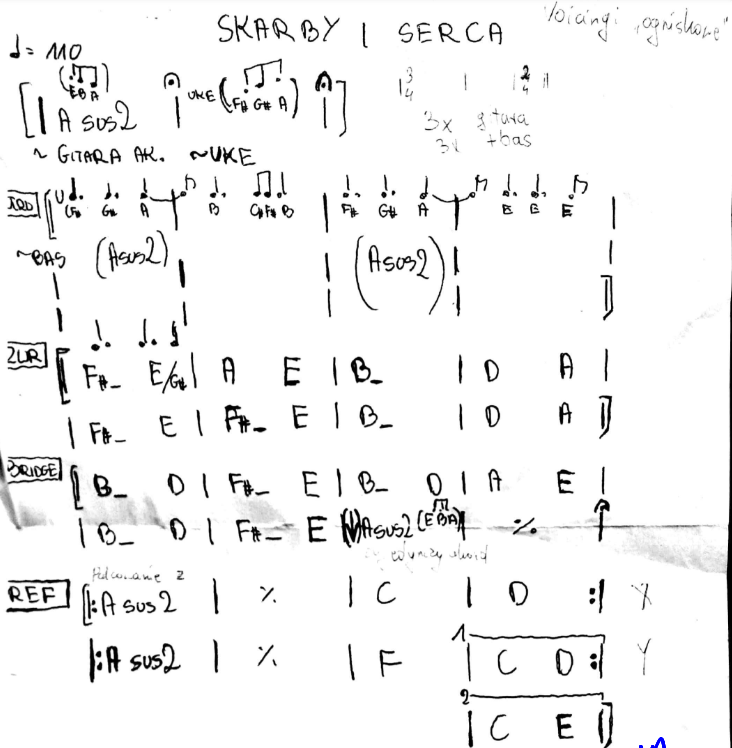
\includegraphics[height=16cm]{images/skarby.png}
    \end{center}
\end{song}
